
\newpage
\section{Injection SQL }


\subsection{Description}
L'injection SQL, en anglais SQL  injection, ou SQLi en abrégé, est une des attaques les plus dangereuses. Comme pour le Cross Site Scripting présenté dans la suite de ce document, il s'agit ici de tirer parti de l'absence de filtrage des entrées utilisateurs. Cette absence de contrôles permet à un hacker d'insérer du code qui sera interprété par l'analyseur cible, par exemple SQL.

\paragraph{}
Dans la cas particulier de l'injection SQL et du site DVWA, les requêtes SQL, imbriquées dans des scripts PHP qui récupèrent les saisies des utilisateurs, peuvent être détournées sur la base de la syntaxe du langage. 




\subsection{Exploitation}

\subsubsection{DVWA - Security level "low"}

La base de données contient 5 utilisateurs identifiés par les entiers de 1 à 5.
La mission proposée par le DVWA est de voler leurs mots de passe par injection SQL.

On règle la "DVWA security" sur low de manière à avoir un site web "damn vulnerable".
On saisit dans le champ User Id, une simple apostrophe i.e. '. Le site retourne le message
"\it {You have an error in your SQL syntax; check the manual that corresponds to your MariaDB server version for the right syntax to use near ''''' at line 1}"

\paragraph{}Cette simple apostrophe démontre que le site est vulnérable pour deux raisons : d'abord on sait que nos saisies sont interprétées directement par l'analyseur SQL ; elle ne sont pas filtrées. Ensuite parce que le site est "bavard".

\begin{figure}[!h]
	\begin{center}
		\label{}
		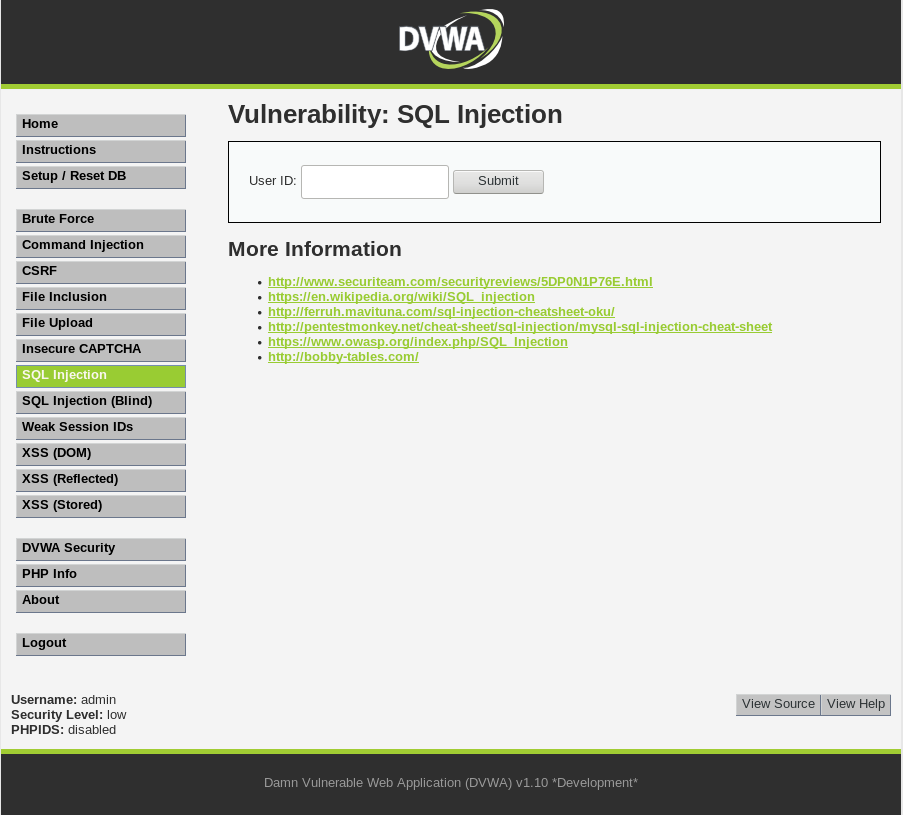
\includegraphics[scale=\scaledvwa]{images/sql/sqli1.png}
		\caption{Les saisies incorrectes donnent lieu à un message d'erreur SQL qui informe le hacker potentiel de l'absence de protection contre les SQLi. D'autres informations importantes sont dévoilées comme le type de base de donnée, ici MariaDB, version libre de MySql rachetée par Oracle.}
	\end{center}
\end{figure}

Un clic sur le bouton "View Source" affiche le code PHP de la page. On constate, en effet, qu'on peut saisir n'importe quoi dans le champ User Id, il sera transmis sans modification à la requête \$query via \$id.   

\begin{figure}[!h]
	\begin{center}
		\label{}
		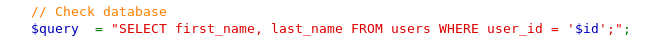
\includegraphics[scale=0.8]{images/sql/code_low.png}
	\end{center}
\end{figure}



\begin{figure}[!h]
	\begin{center}
		\label{}
		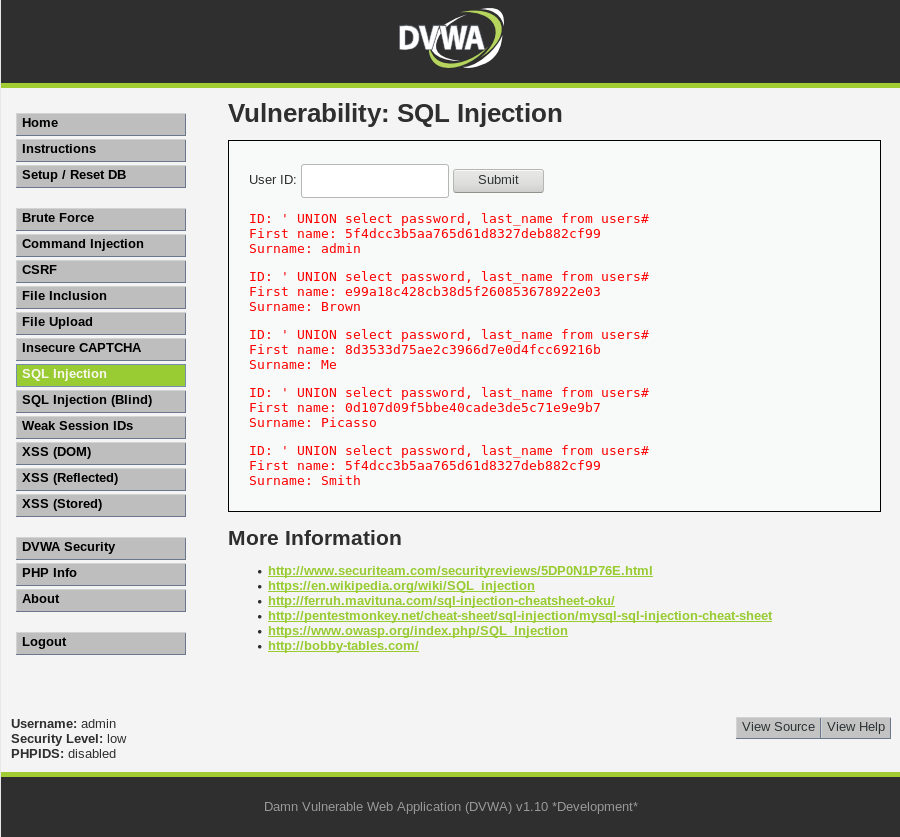
\includegraphics[scale=\scaledvwa]{images/sql/sqli_low.png}
		\caption{Vol des mots de passe par l'injection SQLi sur site non protégé.}
	\end{center}
\end{figure}

L'injection SQL suivante :
{\color{red}

\begin{verbatim}
   ' UNION select password, last_name from users#
\end{verbatim}
}

%  a' UNION SELECT password,last_name from users;-- -&Submit=Submit
% url correspondante 
%  ?id='+UNION+SELECT+password%2Clast_name+from+users%23&Submit=Submit#

donne la requête suivante en remplaçant \$id dans le script PHP :

{\color{red}
\begin{verbatim}
$query  = "SELECT first_name, last_name FROM users WHERE user_id = '' UNION 
           SELECT password, last_name from users#   ';"; 
\end{verbatim}
}
Elle indique donc qu'on effectue l'union au sens mathématique des éléments recueillis par les deux requêtes. Le premier SELECT donne l'ensemble vide, le second donne tous les mots de passe et noms de la table users. On obtient donc les mots de passe faussement associés au champ "First name". Ces mots de passe sont cryptés. On pourra utiliser des techniques de révélation par ingénieurie sociales, recherche internet, force brute, dictionnaires ou rainbow tables. L'outil John the ripper peut entrer en action. On note que Smith est certainement aussi admin car ces deux noms d'utilisateurs ont le même hash donc le même mot de passe. Le hacker peut être confiant quant à la suite des opération car Smith ne semble pas être un adepte de la SSI. Le caractère \# en fin d'injection évite que PHP n'interprête la suite du code en particulier les caractères apostrophes et guillements qui donneraient une erreur SQL.

NB : C'est une technique répandue que de forcer l'analyseur SQL à ignorer le reste de la requête, en utilisant le symbole commentaire SQL double tiret - - les symboles de commentaires PHP dièse \#, {/* */}, {//} pour assurer que ce qui suit l'injection ne sera pas interprété.  



\paragraph{}
Un injection SQL peut aussi donner accès au système de fichier comme le montre l'injection ci-après :
\begin{verbatim} [ ' UNION ALL SELECT load_file('/etc/passwd'),null # ] \end{verbatim}

\begin{figure}[!h]
	\begin{center}
		\label{}
		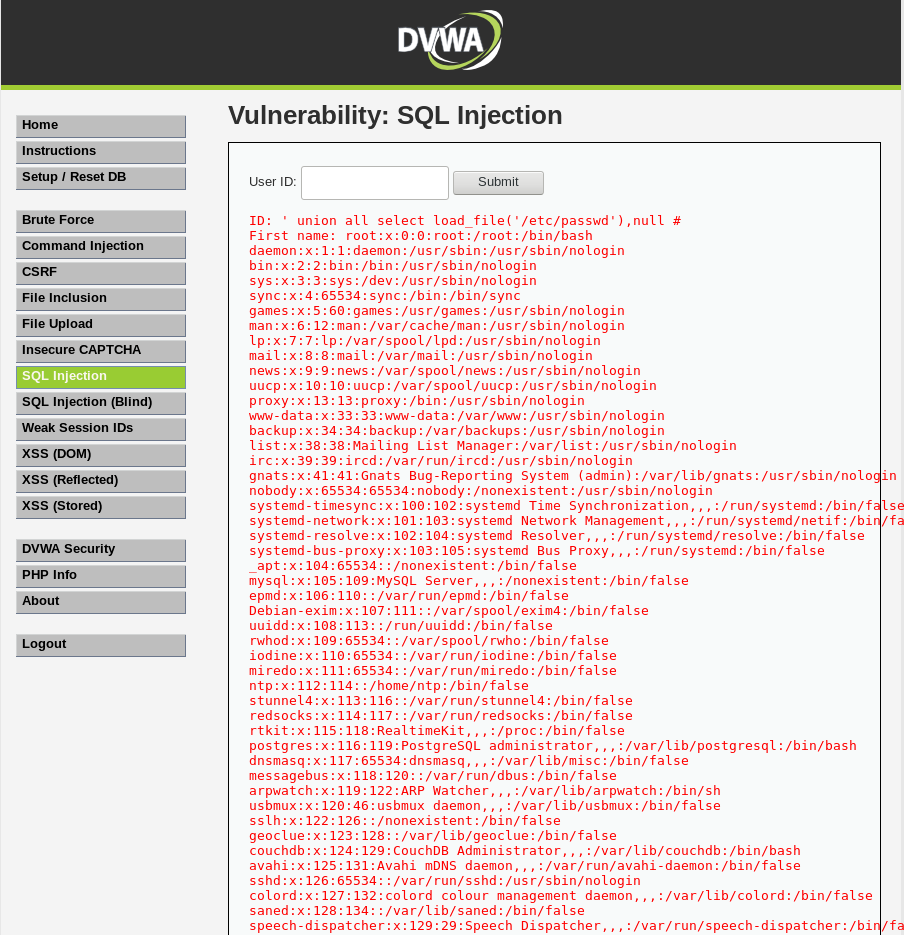
\includegraphics[scale=\scaledvwa]{images/sql/sqli_low2.png}
		\caption{Récupération du fichier /etc/passwd via la commande load\_file : }
	\end{center}
\end{figure}




% ?id=a UNION SELECT password,last_name from users;-- -&Submit=Submit
% ?id=a %27UNION SELECT password,last_name from users#


Si l’on part à la recherche des méthodes et fonctions que l’on peut utiliser en PHP afin de se protéger de certains caractères, on peut croiser le chemin de la fonction PHP mysql\_real\_escape\_string. Celle-ci est souvent utilisée pour protéger les requêtes SQL intégrant des paramètres envoyés par l’utilisateur. Néanmoins nous allons voir que cette fonction peut être déjouée, c’est d’ailleurs le but dans ce niveau DVWA.

Si l’on schématise, il faut donc faire passer des caractères comme des guillemets ou des apostrophes, sans inscrire dans l’URL les caractères en question. Un joyeux défi ! Pour ceux qui ont l’habitude de travailler sur les technos web, vous avez peut être déjà entendu parlé de l’encodage, et plus spécifiquement de l’encodage HTTP ou “HTML URL Encoding”. Pour ceux qui ne voient pas de quoi il s’agit, je vous conseille de faire un tour sur cette page : http://www.w3schools.com/tags/ref\_urlencode.asp

L’HTML URL Encoding permet entre autre de faire passer au travers une URL des caractères spéciaux ou des lettres avec accent qui pourraient ne pas être interprétés correctement par les navigateurs ou les serveurs web. Ainsi, l’utilisation d’un encodage basé sur les caractères ASCII est utilisé (notamment la valeur “Hex” des lettres : http://table-ascii.com/ )

\begin{verbatim}
En utilisant l’HTTP URL Encoding, un espace devient un %20 dans l’URL, un  “!” devient un %21, un “%” un %25, etc.

Cela nous permet donc ici de faire passer une guillemet ou une apostrophe de façon encodée pour ne pas qu’ils soient détectés et échappés par la fonction mysql_real_escape_string.
\end{verbatim}


\subsubsection{DVWA - Security level "Medium" et "High"}

Pour récupérer les mots de passe lorsque l'on règle le niveau de sécurité de DVWA sur "haut" et "medium", on utilise une combinaison des outils "Burp suite" et "sqlmap" fournis par kali linux. Le navigateur doit être configuré en utilisant ce proxy Burp suite, à savoir 127.0.0.1:8080. Cela permet l'interception des requêtes POST qui est alors copiée dans un fichier toto.txt utilisé ensuite dans la commande.

\begin{verbatim}
sqlmap -r ./toto.txt –dbs -D dvwa –dump all –os-shell
\end{verbatim}


\subsection{Contre-mesures}

\begin{figure}[!h]
	\begin{center}
		\label{}
		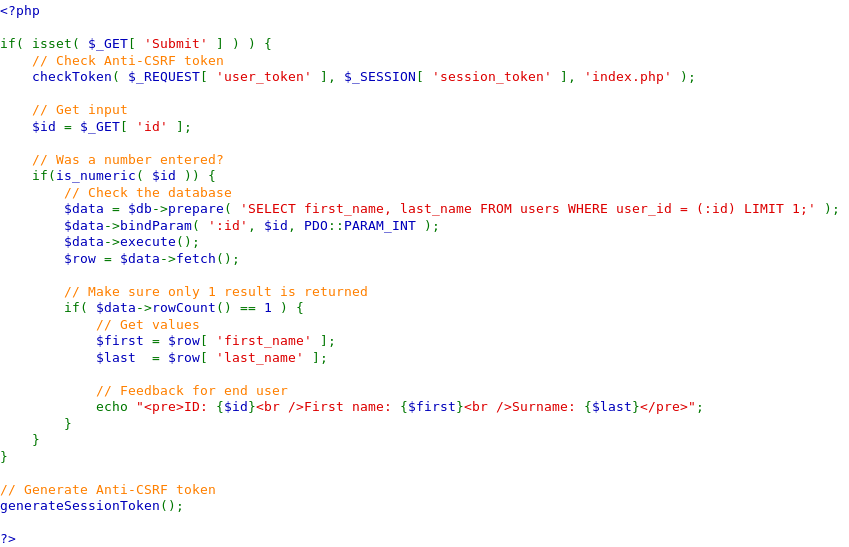
\includegraphics[scale=\scaledvwa]{images/sql/sqli_impossible.png}
		\caption{Récupération du fichier /etc/passwd via la commande load\_file : }
	\end{center}
\end{figure}

The queries are now parameterized queries (rather than being dynamic). This means the query has been defined by the developer, and has distinguish which sections are code, and the rest is data.


\subsubsection{utilisation de }























\section{Injection SQL aveugle}
Blind SQL injection ou BSQLi
\subsection{Description}
When an attacker executes SQL injection attacks, sometimes the server responds with error messages from the database server complaining that the SQL query's syntax is incorrect. Blind SQL injection is identical to normal SQL Injection except that when an attacker attempts to exploit an application, rather then getting a useful error message, they get a generic page specified by the developer instead. This makes exploiting a potential SQL Injection attack more difficult but not impossible. An attacker can still steal data by asking a series of True and False questions through SQL statements, and monitoring how the web application response (valid entry retunred or 404 header set).

"time based" injection method is often used when there is no visible feedback in how the page different in its response (hence its a blind attack). This means the attacker will wait to see how long the page takes to response back. If it takes longer than normal, their query was successful.

\subsection{Exploitation}

\subsection{Contre-mesure}


\section{Attaques XSS }Reflected XSS

\subsection{Description}
 désignées au choix par les acronymes CSS ou XSS et qui seront
Un site web qui fournit d'une part un service de recueille d'informations via des formulaires et d'autre part un service de publication sur le site de ces mêmes informations
\subsection{Exploitation}

\subsection{Contre-mesure}


\section{Attaques XSS enregistrées }

\subsection{Description}

\subsection{Exploitation}

\subsection{Contre-mesure}

%Stored and Reflected XSS Attacks
%
%XSS attacks can generally be categorized into two categories: stored and reflected. There is a third, much less well known type of XSS attack called DOM Based XSS that is discussed seperately here.
%Stored XSS Attacks
%
%Stored attacks are those where the injected script is permanently stored on the target servers, such as in a database, in a message forum, visitor log, comment field, etc. The victim then retrieves the malicious script from the server when it requests the stored information. Stored XSS is also sometimes referred to as Persistent or Type-I XSS.
%Reflected XSS Attacks
%
%Reflected attacks are those where the injected script is reflected off the web server, such as in an error message, search result, or any other response that includes some or all of the input sent to the server as part of the request. Reflected attacks are delivered to victims via another route, such as in an e-mail message, or on some other web site. When a user is tricked into clicking on a malicious link, submitting a specially crafted form, or even just browsing to a malicious site, the injected code travels to the vulnerable web site, which reflects the attack back to the user’s browser. The browser then executes the code because it came from a "trusted" server. Reflected XSS is also sometimes referred to as Non-Persistent or Type-II XSS.
%Other Types of XSS Vulnerabilities
%In addition to Stored and Reflected XSS, another type of XSS, DOM Based XSS was identified by Amit Klein in 2005. OWASP recommends the XSS categorization as described in the OWASP Article: Types of Cross-Site Scripting, which covers all these XSS terms, organizing them into a matrix of Stored vs. Reflected XSS and Server vs. Client XSS, where DOM Based XSS is a subset of Client XSS.
%
%XSS Attack Consequences
%
%
%
%The consequence of an XSS attack is the same regardless of whether it is stored or reflected (or DOM Based). The difference is in how the payload arrives at the server. Do not be fooled into thinking that a “read only” or “brochureware” site is not vulnerable to serious reflected XSS attacks. XSS can cause a variety of problems for the end user that range in severity from an annoyance to complete account compromise. The most severe XSS attacks involve disclosure of the user’s session cookie, allowing an attacker to hijack the user’s session and take over the account. Other damaging attacks include the disclosure of end user files, installation of Trojan horse programs, redirect the user to some other page or site, or modify presentation of content. An XSS vulnerability allowing an attacker to modify a press release or news item could affect a company’s stock price or lessen consumer confidence. An XSS vulnerability on a pharmaceutical site could allow an attacker to modify dosage information resulting in an overdose. For more information on these types of attacks see Content Spoofing.
%How to Determine If You Are Vulnerable
%XSS flaws can be difficult to identify and remove from a web application. The best way to find flaws is to perform a security review of the code and search for all places where input from an HTTP request could possibly make its way into the HTML output. Note that a variety of different HTML tags can be used to transmit a malicious JavaScript. Nessus, Nikto, and some other available tools can help scan a website for these flaws, but can only scratch the surface. If one part of a website is vulnerable, there is a high likelihood that there are other problems as well.
%How to Protect Yourself
%The primary defenses against XSS are described in the OWASP XSS Prevention Cheat Sheet.
%
%
%
%Also, it's crucial that you turn off HTTP TRACE support on all webservers. An attacker can steal cookie data via Javascript even when document.cookie is disabled or not supported on the client. This attack is mounted when a user posts a malicious script to a forum so when another user clicks the link, an asynchronous HTTP Trace call is triggered which collects the user's cookie information from the server, and then sends it over to another malicious server that collects the cookie information so the attacker can mount a session hijack attack. This is easily mitigated by removing support for HTTP TRACE on all webservers.
%
%The OWASP ESAPI project has produced a set of reusable security components in several languages, including validation and escaping routines to prevent parameter tampering and the injection of XSS attacks. In addition, the OWASP WebGoat Project training application has lessons on Cross-Site Scripting and data encoding.


%
%\begin{itemize}
%\item dans le « pire cas » et par le caractère super-croissant de la clé privée, le dernier élément $s_n$ vaudra $D2^{n-1}$ ;
%\item on aura alors $p$ de l'ordre de grandeur de $D2^n$ à $FD2^n$ ;
%\item les éléments de la clé publique $T$ sont majorés par $p$ par le modulo et un bloc chiffré $y$ sera donc borné par $n \times FD2^n$.
%\end{itemize}

%
%\begin{figure}[!h]
%\begin{center}
%\hspace*{-2in}
%  \centering
% 	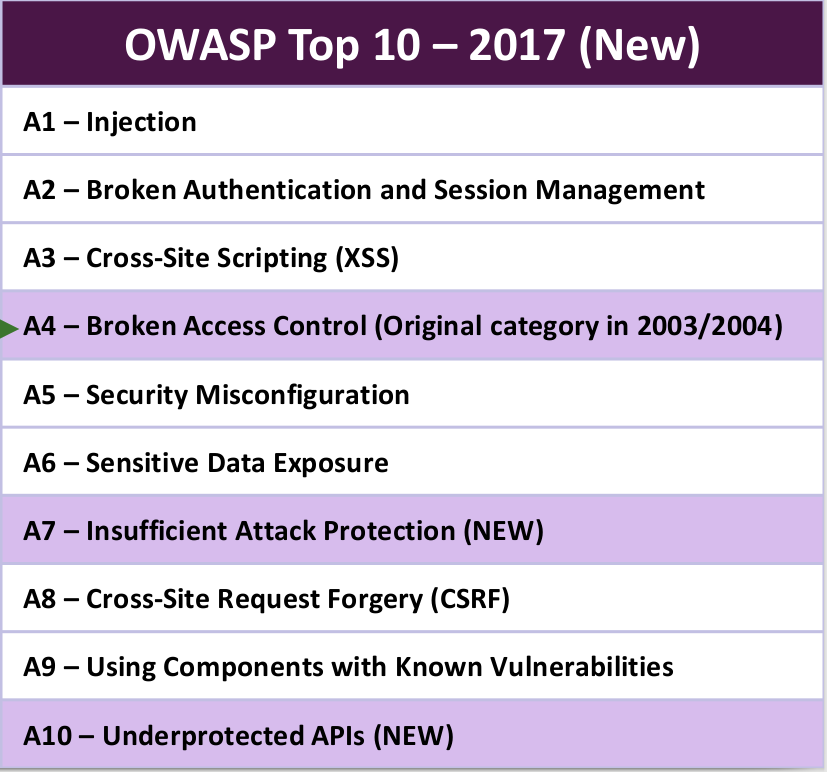
\includegraphics[scale=0.4]{images/10_menaces.png}
%  \caption{Chiffrement d'un flux avec une clé de taille $n = 11$}
%  \label{chiffrement}
%\end{center}
%\end{figure}




%
%
%@ARTICLE{1056964,
%	author={A. Shamir},
%	journal={IEEE Transactions on Information Theory},
%	title={A polynomial-time algorithm for breaking the basic Merkle-Hellman cryptosystem},
%	year={1984},
%	volume={30},
%	number={5},
%	pages={699-704},
%	keywords={Cryptography;Computer science;Graphics;Mathematics;Microcomputers;Polynomials;Protection;Public key;Public key cryptography;Security;Testing},
%	doi={10.1109/TIT.1984.1056964},
%	ISSN={0018-9448},
%	month={Sep},}
%
%
%@BOOK{MARTIN2004,
%	title = {Codage, cryptologie et applications},
%	publisher = {Presses polytechniques et universitaires romandes},
%	year = {2014},
%	author = {Martin, Bruno}
%}
%
%@Book{GJ1979,
%	author = "Michael R. Garey and David S. Johnson",
%	title = "{Computers and Intractability, A Guide to the Theory of {NP}-Completeness}",
%	publisher = "W.H. Freeman and Company",
%	year = 1979,
%	address = "New York"
%}
%
%@book{opac,
%	title = "Handbook of Applied Cryptography",
%	author = "Alfred J. Menezes and Paul C. Van Oorschot and Scott A. Vanstone",
%	publisher = "CRC Press",
%	address = "Boca Raton, London, New York",
%	url = "http://opac.inria.fr/record=b1092394",
%	isbn = "0-8493-8523-7",
%	year = 1996,
%	note = {\url{http://cacr.uwaterloo.ca/hac/}}
%}
%
%@ARTICLE{DEROFF,
%	author={J. Deroff and R. Goyat},
%	title={Le problème du sac à dos en cryptographie},
%	year={2007},
%	note = {\url{http://j.deroff.free.fr/rapportter.pdf}}
%}
%
%@Book{stinson1996,
%	author =       {Stinson, Douglas},
%	title =        {{Cryptographie -- Théorie et pratique}},
%	publisher =    {International Thomson Publishing},
%	year =         {1996},
%	note =         {Traduction de Serge Vaudenay},
%}
%
%@ARTICLE{COSTER,
%	author={Coster, Matthijs J. and Joux, Antoine  and La Macchia, Brian A. and Odlyzko, Andrew M. and Schnorr, Claus-Peter and Stern, Jacques},
%	title={Improved low-density subset sum algorithms},
%	journal={computational complexity},
%	year={1992},
%	volume={2},
%	number={2},
%	pages={111-128},
%	mounth={June},
%	note = {\url{http://www.di.ens.fr/~fouque/ens-rennes/sac-LLL.pdf}}
%}
%
%@article{Merkle,
%	author = {Merkle, R. and Hellman, M.},
%	title = {Hiding Information and Signatures in Trapdoor Knapsacks},
%	journal = {IEEE Trans. Inf. Theor.},
%	issue_date = {1978},
%	volume = {24},
%	number = {5},
%	month = {Sep},
%	year = {1978},
%	issn = {0018-9448},
%	pages = {525--530},
%	numpages = {6},
%	url = {http://dx.doi.org/10.1109/TIT.1978.1055927},
%	doi = {10.1109/TIT.1978.1055927},
%	acmid = {2269393},
%	publisher = {IEEE Press},
%	address = {Piscataway, NJ, USA},
%} 
